\documentclass[aspectratio=169]{beamer}

% The  following themes, you can uncomment it to use
% Want to figure out  what theme you have  on your computer(this refers to linux distro) that you can use
% the following cpmmand may help you:
%
% ls /usr/share/texlive/texmf-dist/tex/latex/beamer | grep "^beamertheme"
%
% Or you can go to:
% https://deic.uab.cat/~iblanes/beamer_gallery/   to see more info

%%%%%%%%%%%%%%%%%%%%%%%%%%%%%%%%%%%%%%%%
% \usetheme[named=mygreen]{Berkeley}
% \usetheme{Warsaw}
 \usetheme{metropolis} % reference:https://mirror.mwt.me/ctan/macros/latex/contrib/beamer-contrib/themes/metropolis/doc/metropolistheme.pdf
% \usetheme{AnnArbor}
% \usetheme{Berlin}
% \usecolortheme{crane}
% \usecolortheme{seahorse}
% \usecolortheme{dolphin}
%%%%%%%%%%%%%%%%%%%%%%%%%%%%%%%%%%%%%%%%

%%%%%%%%%%%%%%%%%%%%%%%%%%%%%%%%%%%%%%%%
% User defined color 
% you can also get more from http://latexcolor.com/
%%%%%%%%%%%%%%%%%%%%%%%%%%%%%%%%%%%%%%%%
\definecolor{mygreen}{rgb}{.125, .5, .25}


%%%%%%%%%%%%%%%%%%%%%%%%%%%%%%%%%%%%%%%%
% support for chinese
%%%%%%%%%%%%%%%%%%%%%%%%%%%%%%%%%%%%%%%%
\usepackage{ctex}

%%%%%%%%%%%%%%%%%%%%%%%%%%%%%%%%%%%%%%%%
% support for images and set the image path
%%%%%%%%%%%%%%%%%%%%%%%%%%%%%%%%%%%%%%%%
\usepackage{graphicx}
\graphicspath{ {./images/} }


%%%%%%%%%%%%%%%%%%%%%%%%%%%%%%%%%%%%%%%%
% support for table
%%%%%%%%%%%%%%%%%%%%%%%%%%%%%%%%%%%%%%%%
\usepackage{multirow}



\begin{document}
%
% Basic Information Of This Silde
%

\title{计算机素质基础|深圳市考 | 安徽计算机专业测试}
\author{小刘}
\institute{公考}
\date{\today}

%%%%%%%%%%%%%%%%%%%%%%%%%%%%%%%%%%%%%%%%
% titlepage
%%%%%%%%%%%%%%%%%%%%%%%%%%%%%%%%%%%%%%%%
\begin{frame}
\titlepage
\end{frame}

%%%%%%%%%%%%%%%%%%%%%%%%%%%%%%%%%%%%%%%%
% A frame
%%%%%%%%%%%%%%%%%%%%%%%%%%%%%%%%%%%%%%%%
\begin{frame}[t]{1. 计算机基础知识} \vspace{20pt}
    1.1 计算机的发展

    \begin{enumerate}
        \item{世界上第一台计算机 ENIAC, 1946 年 2 月诞生于美国。}
            发展阶段:
        \item{第一代为 1946-1957 年,电子管计算机:数据处理;}
        \item{第二代为 1958-1964 年,晶体管计算机:工业控制;}
        \item{第三代为 1965-1971 年,中小规模集成电路:小型计算机;}
        \item{第四代为 1972 迄今,大规模和超大规模集成电路:微型计算机;}
            CPU:
        \item{1971 年 Intel 公司开发出 Intel 4004(第一块 CPU)微处理器,标志进入了微型
机阶段。}\\
\textbf{电子 -> 晶体 -> 中小集成 -> 大规模集成}

    \end{enumerate}

\end{frame}


%%%%%%%%%%%%%%%%%%%%%%%%%%%%%%%%%%%%%%%%
% A frame
%%%%%%%%%%%%%%%%%%%%%%%%%%%%%%%%%%%%%%%%
\begin{frame}[t]{1. 计算机基础知识} \vspace{20pt}
    1.2 我国计算机的发展

    \begin{enumerate}
        \item{1958 年 我国研制成功第一台计算机 103 机;}
        \item {1983 年 国防科技大学研制成功的银河-I 号亿次运算巨型计算机是我国自行研制的
第 1 台亿次运算计算机系统;
}
        \item {2009 年 曙光 5000A,峰值计算速度超过 200 万亿次(我国首台百万亿次超级计算机);}
        \item {2009 年 11 月 “天河一号”的峰值速度达到每秒 1206.19 万亿次,是中国首台每秒运
算速度超过千万亿次的超级计算机。
}
        \item {2010 年 “天河一号”升级后的“天河一号 A” 的峰值速度达到每秒 2570 万亿次,
速度超过当时的最快的超级计算机—美国的“美洲豹”(每秒 1750 万亿次),
成为当时世界上运算速度最快的计算机。}
    \end{enumerate}

\end{frame}

%%%%%%%%%%%%%%%%%%%%%%%%%%%%%%%%%%%%%%%%
% A frame
%%%%%%%%%%%%%%%%%%%%%%%%%%%%%%%%%%%%%%%%
\begin{frame}[t]{1. 计算机基础知识} \vspace{20pt}
    1.3 计算机的分类

    \begin{enumerate}
        \item{按用途分}\\
            通用计算机\\
            专用计算机\\
        \item{按规模及性能分} \\
            巨型计算机\\
            大/中型计算机\\
            小型计算机\\
            微型计算机\\
            工作站和服务器。\\
        \item{ 按计算机的原理分类:模拟式电子计算机、数字电子计算机和数字模拟混合式电子计算机}
    \end{enumerate}

\end{frame}

%%%%%%%%%%%%%%%%%%%%%%%%%%%%%%%%%%%%%%%%
% A frame
%%%%%%%%%%%%%%%%%%%%%%%%%%%%%%%%%%%%%%%%
\begin{frame}[t]{1. 计算机基础知识} \vspace{20pt}
    1.4 计算机的特点
            自动控制能力;\\
            处理速度快、精度高;\\
            “记忆”能力强;\\
            能进行逻辑判断;\\
            很高的计算精度;\\
            支持人机交互;通用性强。\\
            支持人机交互;通用性强。\\
            计算机的体系结构仍在继续发展,其发展趋势是智、多、网、巨、微。\\
\end{frame}

%%%%%%%%%%%%%%%%%%%%%%%%%%%%%%%%%%%%%%%%
% A frame
%%%%%%%%%%%%%%%%%%%%%%%%%%%%%%%%%%%%%%%%
\begin{frame}[t]{1. 计算机基础知识} \vspace{20pt}
    1.5 计算机的主要应用领域

    \begin{enumerate}
        \item{科学计算:最早的应用领域}\\ 如导弹的发射,宇宙飞船的飞行轨迹计算等。
        \item{数据处理(信息处理):最广泛的应用领域} 
            \\包括对数据的收集、记载、分类、排序、检索、计算或加工、传输、制 表等工作。
            例如,在科研、生产和经济活动中,把所获得的大量信息存入计算机,通过加工处理,
            得到可供某种目的使用的新信息。
        \item{实时控制}\\ 常用于电力、冶金、石油化工、机械等工业。
        \item{计算机辅助} \\ 计算机辅助设计(CAD);计算机辅助制造(CAM)
            计算机辅助教学(CAI);计算机辅助测试(CAT)
    \end{enumerate}

\end{frame}

%%%%%%%%%%%%%%%%%%%%%%%%%%%%%%%%%%%%%%%%
% A frame
%%%%%%%%%%%%%%%%%%%%%%%%%%%%%%%%%%%%%%%%
\begin{frame}[t]{1. 计算机基础知识} \vspace{20pt}

    练习题\\
        1. 世界上第一台电子计算机诞生于(    )\\
            A. 1945 年\\
            B. 1946 年\\
            C. 1949 年\\
            D. 1950 年\\

\end{frame}

%%%%%%%%%%%%%%%%%%%%%%%%%%%%%%%%%%%%%%%%
% A frame
%%%%%%%%%%%%%%%%%%%%%%%%%%%%%%%%%%%%%%%%
\begin{frame}[t]{1. 计算机基础知识} \vspace{20pt}

    练习题\\
            2. 计算机发展过程按使用的电子器件可划分为四代,微型计算机出现在第( )代。\\
            A. 1\\
            B. 2\\
            C. 3\\
            D. 4\\
\end{frame}


%%%%%%%%%%%%%%%%%%%%%%%%%%%%%%%%%%%%%%%%
% A frame
%%%%%%%%%%%%%%%%%%%%%%%%%%%%%%%%%%%%%%%%
\begin{frame}[t]{1. 计算机基础知识} \vspace{20pt}

    练习题\\
            3. 2009 年 6 月 15 日下午,中国首台国产百万亿次超级计算机,每秒峰值计算
速度超过( )万亿次的曙光 5000A—“魔方”在上海超级计算中心正式启用,这标
志着中国已成为继美国之后的一个研发、制造并部署百万亿次超级计算机的国家。

            A. 100\\
            B. 150\\
            C. 200\\
            D. 250\\
\end{frame}

%%%%%%%%%%%%%%%%%%%%%%%%%%%%%%%%%%%%%%%%
% A frame
%%%%%%%%%%%%%%%%%%%%%%%%%%%%%%%%%%%%%%%%
\begin{frame}[t]{1. 计算机基础知识} \vspace{20pt}

    练习题\\
    4.计算机应用最广泛的领域是( )\\
    A. 科学计算\\
    B. 信息处理\\
    C. 过程控制 \\
    D. 人工智能\\

\end{frame}



%%%%%%%%%%%%%%%%%%%%%%%%%%%%%%%%%%%%%%%%
% A frame 
%%%%%%%%%%%%%%%%%%%%%%%%%%%%%%%%%%%%%%%%
\begin{frame}[t]{2. 计算机系统的组成} \vspace{20pt}

    计算机的组成\\
    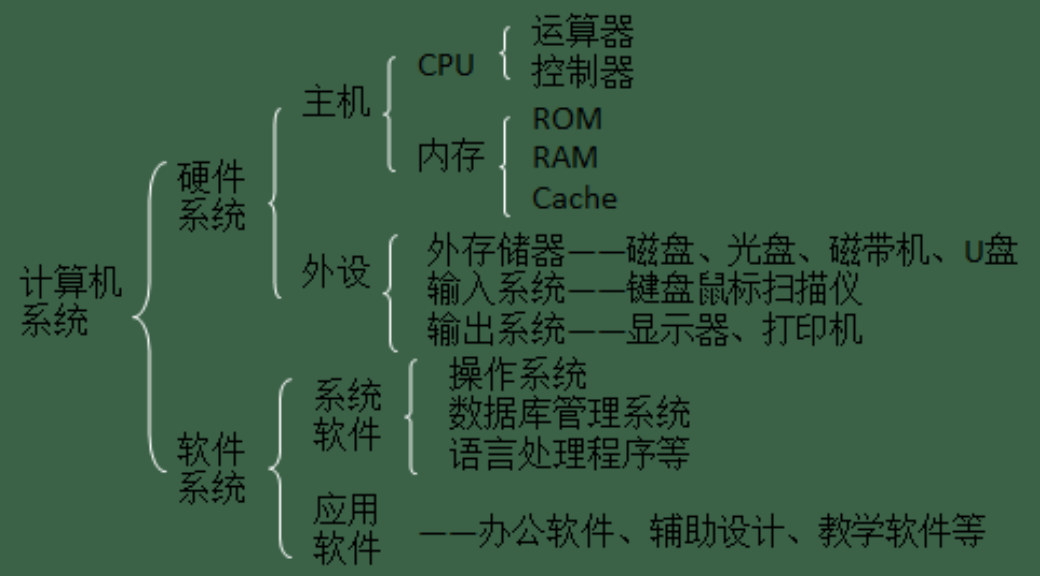
\includegraphics[scale=0.25]{computer_hardware}\\ 
    NOTE: \\
    \textbf{ROM} ||  \textbf{RAM}\\
    \textbf{cache} 
    \textbf{DMA} 
\end{frame}



%%%%%%%%%%%%%%%%%%%%%%%%%%%%%%%%%%%%%%%%
% A frame 
%%%%%%%%%%%%%%%%%%%%%%%%%%%%%%%%%%%%%%%%
\begin{frame}[t]{2. 计算机系统的组成} \vspace{20pt}
    2.1 计算机硬件的概念

    \begin{enumerate}
        \item{计算机硬件(Computer hardware)是指计算机系统中由电子、机械和光电元件等组
            成的各种物理装置的总称}\\
        \item {冯·诺依曼 体系结构}\\
        \item {冯·诺依原理核心思想}\\
            (1)使用二进制;\\
            (2)存储程序和程序控制;\\
            (3)一个完整的计算机硬件系统应该由五个部分组成:运算器、控制器、存储器、
            输入设备、输出设备。\\
    \end{enumerate}

\end{frame}


%%%%%%%%%%%%%%%%%%%%%%%%%%%%%%%%%%%%%%%%
% A frame 
%%%%%%%%%%%%%%%%%%%%%%%%%%%%%%%%%%%%%%%%
\begin{frame}[t]{2. 计算机系统的组成} \vspace{20pt}
    2.2 计算机硬件的各部分功能\\
    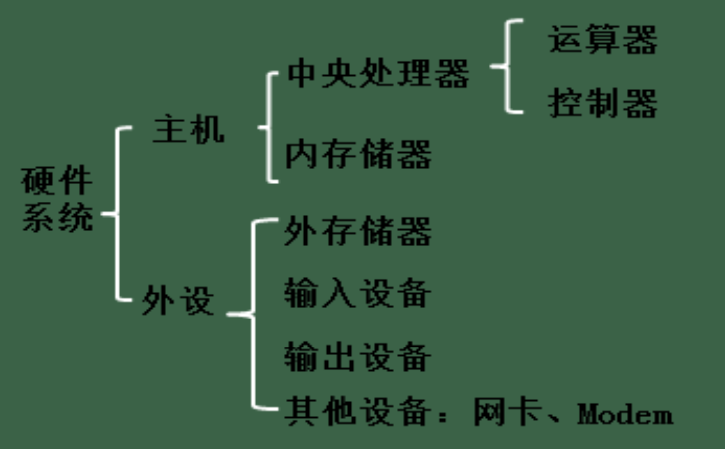
\includegraphics[scale=0.25]{hardware_function}\\ 
\end{frame}

%%%%%%%%%%%%%%%%%%%%%%%%%%%%%%%%%%%%%%%%
% A frame 
%%%%%%%%%%%%%%%%%%%%%%%%%%%%%%%%%%%%%%%%
\begin{frame}[t]{2. 计算机系统的组成} \vspace{20pt}
    2.2 计算机硬件的各部分功能
    \begin{enumerate}
        \item {运算器}\\
            运算器是计算机对数据进行加工处理的中心,对二进制数码进行算术运算或逻辑运
算。\\
计算机的运算速度通常是指每秒钟能够执行加法指令的数目。通常用百万次/每秒
(MIPS)来表示。\\

\item {控制器:}\\
    控制器是计算机的控制中心,由它指挥各个部件自动、协调地工作。\\

    \textbf{运算器 + 控制器 = 中央处理器(CPU)}

\item {存储器:}\\
    存储器是计算机中存放所有数据和程序的记忆部件,它的基本功能是按指定的地址存
(写)入或者取(读)出信息。\\


    \end{enumerate}
\end{frame}


%%%%%%%%%%%%%%%%%%%%%%%%%%%%%%%%%%%%%%%%
% A frame 
%%%%%%%%%%%%%%%%%%%%%%%%%%%%%%%%%%%%%%%%
\begin{frame}[t]{2. 计算机系统的组成} \vspace{20pt}
\textbf{换算关系:}\\
字节、字、位、比特,这四者之间的关系是:\\

    1位=1比特(bit)\\
    1字节(byte)=8位(bit)\\
    1字=2字节(byte)\\
    1字=16位(bit)\\ 

    01|11|00|01||01|01|01|00\\
    0:===================> 1位/1比特 (bit)\\
    01|11|00|01:=============> 1 字节(byte) = 8 比特(bit)\\
    01|11|00|01||01|01|01|00 :======> 1 字 = 2 字节(byte) = 16 位(bit)\\
\end{frame}



%%%%%%%%%%%%%%%%%%%%%%%%%%%%%%%%%%%%%%%%
% A frame 
%%%%%%%%%%%%%%%%%%%%%%%%%%%%%%%%%%%%%%%%
\begin{frame}[t]{2. 计算机系统的组成} \vspace{20pt}
    \textbf{ROM || RAM || CACHE}\\
    a)只读存储器(ROM):是一种只能读出事先所存数据的固态半导体存储器。其特性
是一旦储存资料就无法再将之改变或删除。通常用在不需经常变更资料的电子或电脑
系统中,并且资料不会因为电源关闭而消失。\\
b)随机存储器(RAM):可以被 CPU 随机地读写,故又称为读写存储器。这种存储器
用于存放用户装入的程序、数据及部分系统信息。当机器断电后,所有信息全部丢失。\\
c)高速缓冲存储器(CACHE):用于临时存储频繁使用的信息以加快访问速度。在计
算机存储系统的层次结构中,介于中央处理器和主存储器之间的高速小容量存储器。\\

\textit{外存储器(辅助存储器):简称外存或副存。CPU 不可直接访问其的数据,只
有先调入内存方可使用。例如:硬盘、U 盘、光盘、软盘}\\
\end{frame}


%%%%%%%%%%%%%%%%%%%%%%%%%%%%%%%%%%%%%%%%
% A frame 
%%%%%%%%%%%%%%%%%%%%%%%%%%%%%%%%%%%%%%%%
\begin{frame}[t]{2. 计算机系统的组成} \vspace{20pt}
    
    4.输入设备:\\
    功能:\\
    向计算机输入命令、程序、数据等信息。把这些信息转换为计算机能识别的二
进制代码。\\

例子:\\
    键盘、鼠标、扫描仪、手写板、麦克、照相机、摄像机、游戏操作杆、条形码
阅读器、光学字符阅读器、触摸屏、光笔等。\\

5.输出设备\\
功能:将计算机处理后的各种内部格式信息转换为人们能识别的形式表达出来。\\
例子:显示器、打印机、绘图仪、音响等。\\
\end{frame}


%%%%%%%%%%%%%%%%%%%%%%%%%%%%%%%%%%%%%%%%
% A frame 
%%%%%%%%%%%%%%%%%%%%%%%%%%%%%%%%%%%%%%%%
\begin{frame}[t]{2. 计算机系统的组成} \vspace{20pt}
    2.3 微型计算机的主要技术指标\\
    \begin{enumerate}
        \item{字长:CPU 一次能同时处理二进制数据的位数。}\\
        \item{.时钟主频:指 CPU 的时钟频率,单位 GHz。}\\
            主频=外频*倍频\\
        \item{运算速度:指每秒钟所能执行加法指令数目,常用 MIPS 表示。}\\
        \item{存储容量:主要指内存的存储容量。}\\
        \item{存取周期:指 CPU 从内存储器中存取数据所需要的时间。}\\

    \end{enumerate}

\end{frame}




%%%%%%%%%%%%%%%%%%%%%%%%%%%%%%%%%%%%%%%%
% A frame 
%%%%%%%%%%%%%%%%%%%%%%%%%%%%%%%%%%%%%%%%
\begin{frame}[t]{2. 计算机系统的组成} \vspace{20pt}
    练习题\\
    【单选】1. 冯 · 诺依曼理论的核心是存储程序和( )\\
    A. 顺序存储\\ B. 程序控制\\
    C. 集中存储\\ D. 运算存储分离\\


\end{frame}



%%%%%%%%%%%%%%%%%%%%%%%%%%%%%%%%%%%%%%%%
% A frame 
%%%%%%%%%%%%%%%%%%%%%%%%%%%%%%%%%%%%%%%%
\begin{frame}[t]{2. 计算机系统的组成} \vspace{20pt}
    练习题\\
    【多选】计算机在工作过程中突然断电,不会丢失所保存信息的存储介质是( )\\
    A. 光盘 \\
    B. 硬盘\\
    C. 只读存储器\\
    D. 内存\\
    答案:ABC\\


\end{frame}


%%%%%%%%%%%%%%%%%%%%%%%%%%%%%%%%%%%%%%%%
% A frame 
%%%%%%%%%%%%%%%%%%%%%%%%%%%%%%%%%%%%%%%%
\begin{frame}[t]{2. 计算机系统的组成} \vspace{20pt}
    练习题\\
    【单选】微机中 1K 字节表示的二进制位数是( )\\
A. 1000\\
B. 8×1000\\
C. 1024\\
D. 8×1024\\
\end{frame}



%%%%%%%%%%%%%%%%%%%%%%%%%%%%%%%%%%%%%%%%
% A frame 
%%%%%%%%%%%%%%%%%%%%%%%%%%%%%%%%%%%%%%%%
\begin{frame}[t]{2. 计算机系统的组成} \vspace{20pt}
    练习题\\
    【单选】微机中 1K 字节表示的二进制位数是( )\\
A. 1000\\
B. 8×1000\\
C. 1024\\
D. 8×1024\\
1k = 1024 字节 = 8 * 1024 字/bit/比特/二进制位数\\
答案:D\\
\end{frame}


%%%%%%%%%%%%%%%%%%%%%%%%%%%%%%%%%%%%%%%%
% A frame 
%%%%%%%%%%%%%%%%%%%%%%%%%%%%%%%%%%%%%%%%
\begin{frame}[t]{2. 计算机系统的组成} \vspace{20pt}
    练习题\\
    【多选】 下列属于输入设备的是( )\\
    A. 鼠标\\ B. 打印机\\
    C. 扫描仪\\ D. 显示器\\
    答案:AC\\
\end{frame}



%%%%%%%%%%%%%%%%%%%%%%%%%%%%%%%%%%%%%%%%
% A frame 
%%%%%%%%%%%%%%%%%%%%%%%%%%%%%%%%%%%%%%%%
\begin{frame}[t]{3. 计算机软件的概念及分类} \vspace{20pt}
    3.1. \textbf{概念}\\
    计算机软件(Computer Software)是指计算机系统中的程序、数据及其文档。软
件是用户与硬件之间的接口界面。用户主要是通过软件与计算机进行交流。
\end{frame}




%%%%%%%%%%%%%%%%%%%%%%%%%%%%%%%%%%%%%%%%
% A frame 
%%%%%%%%%%%%%%%%%%%%%%%%%%%%%%%%%%%%%%%%
\begin{frame}[t]{3. 计算机软件的概念及分类} \vspace{20pt}
    3.2. \textbf{软件的分类}\\
    |\\
    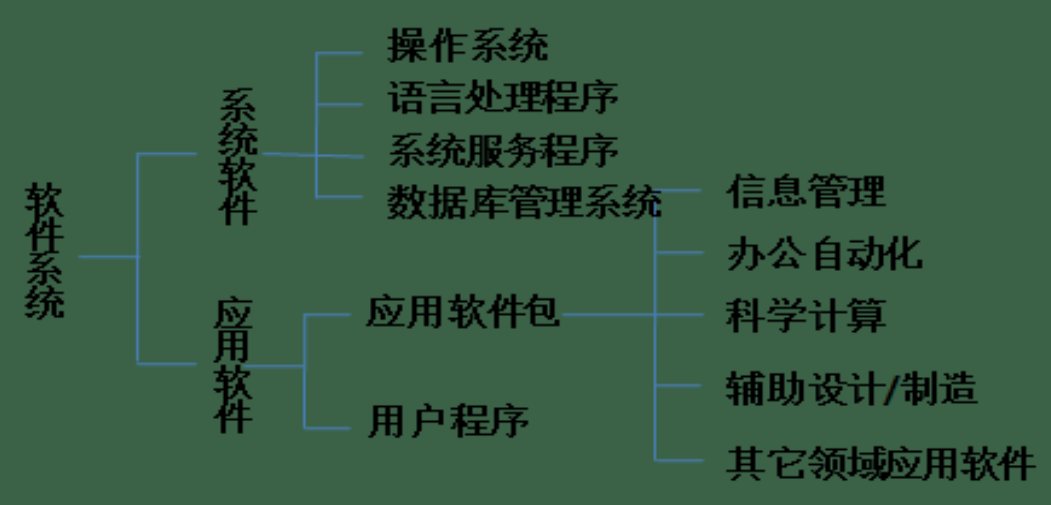
\includegraphics[scale=0.3]{computer_software}\\ 
\end{frame}


%%%%%%%%%%%%%%%%%%%%%%%%%%%%%%%%%%%%%%%%
% A frame 
%%%%%%%%%%%%%%%%%%%%%%%%%%%%%%%%%%%%%%%%
\begin{frame}[t]{3. 计算机软件的概念及分类} \vspace{20pt}
    \begin{enumerate}
        \item{系统软件}\\
            指控制和协调计算机及外部设备,支持应用软件开发和运行的系统,是无需用户干
预的各种程序的集合,主要功能是调度,监控和维护计算机系统;负责管理计算机系
统中各种独立的硬件,使得它们可以协调工作。\\

        \item{应用软件}\\
            在计算机硬件和系统软件的支持下,为解决各类专业和实际问题而设计开发的一
类软件。如杀毒软件、文字处理、电子表格、多媒体制作工具、各种工程设计和数学
计算软件、模拟过程、辅助设计和管理程序等。\\
        \item{程序设计语言}: 人们让计算机完成某项任务的语言\\
            1)机器语言:直接执行\\
2)汇编语言:符号语言,需要编译才能执行\\
3)高级语言:接近自然语言(编译方式和解释方式执行)\\
    \end{enumerate}

\end{frame}

%%%%%%%%%%%%%%%%%%%%%%%%%%%%%%%%%%%%%%%%
% A frame 
%%%%%%%%%%%%%%%%%%%%%%%%%%%%%%%%%%%%%%%%
\begin{frame}[t]{3. 计算机软件的概念及分类} \vspace{20pt}
    练习题:\\
    【多选】下列选项中属于系统软件的是( )\\
A. 数据库管理系统\\ B. 操作系统\\
C. 语言处理系统\\ D. 用户应用程序\\
答案:ABC\\
\end{frame}



%%%%%%%%%%%%%%%%%%%%%%%%%%%%%%%%%%%%%%%%
% A frame 
%%%%%%%%%%%%%%%%%%%%%%%%%%%%%%%%%%%%%%%%
\begin{frame}[t]{3. 计算机软件的概念及分类} \vspace{20pt}
    练习题:\\
    【单选】计算机软件系统包括( )\\
A.系统软件和应用软件\\
B. 编辑软件和应用软件\\
C. 数据库软件和工具软件\\
D. 程序和数据\\
答案:A\\
\end{frame}

%%%%%%%%%%%%%%%%%%%%%%%%%%%%%%%%%%%%%%%%
% A frame 
%%%%%%%%%%%%%%%%%%%%%%%%%%%%%%%%%%%%%%%%
\begin{frame}[t]{4. 计算机中常用的数制及相互转换} \vspace{20pt}
    \textbf{数制基本概念:}\\
    数的表示规则。通常按进位原则进行计数。称为进位计数制,简称数制。人们通
    常采用的数制有十进制、二进制、八进制和十六进制。数制的表示主要包括三个基本
    要素:数码、基数和位权。\\

    \textbf{数码:}是指数制中表示基本数值大小的不同数字符号。\\
    \textbf{基数:}是指数制所使用数码的个数。如 R 进制表示有 R 个基本符号,其基数就为 R。\\
    \textbf{位权:}是指数制中某一位上的 1 所表示数值的大小。\\ 
\end{frame}


%%%%%%%%%%%%%%%%%%%%%%%%%%%%%%%%%%%%%%%%
% A frame 
%%%%%%%%%%%%%%%%%%%%%%%%%%%%%%%%%%%%%%%%
\begin{frame}[t]{4. 计算机中常用的数制及相互转换} \vspace{20pt}

    \begin{tabular}{ |p{2cm}|p{1cm}|p{5cm}|p{1cm}|p{3cm}|  }
        \hline
        \multicolumn{5}{|c|}{数制} \\
        \hline
        进位制  & 基数 & 基本符号(数码)& 权 & 表示\\
        \hline
        二进制  & 2    &     0、1 &                                               2  & B (Binary)\\
        八进制  & 8    &     0、1、2、3、4、5、6、7 &                             8  & O(Octal)\\
        十进制  & 10   &     0、1、2、3、4、5、6、7、8、9 &                       10 & D(Decimal)\\
        十六进制& 16   &     0、1、2、3、4、5、6、7、8、9、A、B、C、D、E、C、F &  16 & H (Hexadecimal)\\
        \hline
    \end{tabular}
\end{frame}


%%%%%%%%%%%%%%%%%%%%%%%%%%%%%%%%%%%%%%%%
% A frame
%%%%%%%%%%%%%%%%%%%%%%%%%%%%%%%%%%%%%%%%
\begin{frame}[t]{4. 计算机中常用的数制及相互转换} \vspace{20pt}
    进制转换:\\
... 0011101\\
... 64 32 16 8 4 2 1 \\
... 0  0  1  1 1 0 1\\
... 0+ 0+ 16+8+4+0+1 =29 \\

八进制  \\
... 1  0  3\\
... 64 8 1 \\
... 64+0+3 = 67 \\

十进制..  \\
十六进制..\\

\end{frame}



%%%%%%%%%%%%%%%%%%%%%%%%%%%%%%%%%%%%%%%%
% A frame
%%%%%%%%%%%%%%%%%%%%%%%%%%%%%%%%%%%%%%%%
\begin{frame}[t]{4. 计算机中常用的数制及相互转换} \vspace{20pt}
    练习\\
    【单选】二进制数 1011+1001=( )。\\
A. 10100\\ B. 10101\\
C. 11010\\ D. 10010\\
\end{frame}


%%%%%%%%%%%%%%%%%%%%%%%%%%%%%%%%%%%%%%%%
% A frame
%%%%%%%%%%%%%%%%%%%%%%%%%%%%%%%%%%%%%%%%
\begin{frame}[t]{4. 计算机中常用的数制及相互转换} \vspace{20pt}
    练习\\
    下面几个不同进制数中,最大的数是( )。\\
A. 1100010B\\ B. 25D\\
C. 17O\\ D. 2FDH\\
答案:D\\

\end{frame}



%%%%%%%%%%%%%%%%%%%%%%%%%%%%%%%%%%%%%%%%
% A frame
%%%%%%%%%%%%%%%%%%%%%%%%%%%%%%%%%%%%%%%%
\begin{frame}[t]{4. 计算机中常用的数制及相互转换} \vspace{20pt}
    练习\\
    有一个数制 311 与十六进制数 C9 相等,则该数值是( )数。\\
A. 二进制\\ B. 八进制\\
C. 五进制\\ D. 十六进制\\
答案:B\\
\end{frame}




%%%%%%%%%%%%%%%%%%%%%%%%%%%%%%%%%%%%%%%%
% A frame
%%%%%%%%%%%%%%%%%%%%%%%%%%%%%%%%%%%%%%%%
\begin{frame}[t]{5. 计算机编码} \vspace{20pt}
    5.1 英文字符编码

    \begin{enumerate}
        \item{BCD 码} \\
            计算机将十进制和二进制的转换常用的转换方式是 BCD 码。BCD 码的编码方式有很多,
            有 8421BCD 码、2421BCD 码、余 3 码、格雷码等,最常用的时 8421BCD 码。\\
            BCD 码这种编码形式利用了四个位元来储存一个十进制的数码,使二进制和十进制之
            间的转换得以快捷的进行。例如十进制数 82.5 对应的 BCD 码为(10000010.0101)BCD,
            其码并非真实意义的二进制,对应的二进制数是(1010010.1)2。\\



        \item{ASCII 码} \\
            ASCII 码使用指定 7 位或 8 位二进制数组合来表示 128 或 256 种可能的字符\\
            要记住的几个字符的编码值:\\
            a 字符编码为 1100001,对应十进制为 97,则 b 的编码值为 98。\\
            A 字符编码为 1000001,对应十进制为 65,则 B 的编码值为 66。\\
            0 数字字符编码为 0110000,对应十进制为 48,则 1 的编码值为 49\\
    \end{enumerate}

\end{frame}


%%%%%%%%%%%%%%%%%%%%%%%%%%%%%%%%%%%%%%%%
% A frame
%%%%%%%%%%%%%%%%%%%%%%%%%%%%%%%%%%%%%%%%
\begin{frame}[t]{5. 计算机编码} \vspace{20pt}
    5.2 汉字编码\\
    计算机中汉字的表示也是用二进制编码,一个汉字=两个字节。根据应用目的的
不同,汉字编码分为外码、交换码、机内码和字形码。\\
    \begin{enumerate}
        \item{外码(输入码)} 外码也叫输入码,是用来将汉字输入到计算机中的一组键盘符号。目前常用的输
入码有拼音码、五笔字型码、自然码、表形码、认知码、区位码和电报码等。
        \item{交换码}\\
            计算机内部处理的信息,都是用二进制代码表示的,汉字也不例外。而二进制代
码使用起来是不方便的,于是需要采用信息交换码。中国标准总局 1981 年制定了中
            华人民共和国国家标准 GB2312(80)《信息交换用汉字编码字符集(基本集)》,即国标
码。\\

    \end{enumerate}
\end{frame}


%%%%%%%%%%%%%%%%%%%%%%%%%%%%%%%%%%%%%%%%
% A frame
%%%%%%%%%%%%%%%%%%%%%%%%%%%%%%%%%%%%%%%%
\begin{frame}[t]{5. 计算机编码} \vspace{20pt}

    3. 机内码\\
    根据国标码的规定,每一个汉字都有了确定的二进制代码,在微机内部汉字代码
    都用机内码,在磁盘上记录汉字代码也使用机内码。\\
    4. 汉字的字形码\\

    字形码是汉字的输出码,输出汉字时都采用图形方式,无论汉字的笔画多少,每
    个汉字都可以写在同样大小的方块中。通常用 16×16 点阵来显示汉字。\\
\end{frame}



%%%%%%%%%%%%%%%%%%%%%%%%%%%%%%%%%%%%%%%%
% A frame
%%%%%%%%%%%%%%%%%%%%%%%%%%%%%%%%%%%%%%%%
\begin{frame}[t]{5. 计算机编码} \vspace{20pt}
    练习题\\
    【单选】26 的压缩 BCD 码是( )。\\

    A.00100110 \\B.01100010\\
    C.01100001\\ D.00100100\\
\end{frame}



%%%%%%%%%%%%%%%%%%%%%%%%%%%%%%%%%%%%%%%%
% A frame
%%%%%%%%%%%%%%%%%%%%%%%%%%%%%%%%%%%%%%%%
\begin{frame}[t]{5. 计算机编码} \vspace{20pt}
    练习题\\
    【单选】26 的压缩 BCD 码是( )。\\
    A.00100110 \\B.01100010\\
    C.01100001\\ D.00100100\\

    ==================\\
    2 和 6  分开  表示
0000 0000 \\
0010 0110\\
2 6\\

    答案:A\\
\end{frame}



%%%%%%%%%%%%%%%%%%%%%%%%%%%%%%%%%%%%%%%%
% A frame
%%%%%%%%%%%%%%%%%%%%%%%%%%%%%%%%%%%%%%%%
\begin{frame}[t]{5. 计算机编码} \vspace{20pt}
    练习题\\
    【单选】下列字符中,ASCII 码值最小的是( )。\\
A. a\\ B. A\\
C. x\\ D. Y\\
\end{frame}



%%%%%%%%%%%%%%%%%%%%%%%%%%%%%%%%%%%%%%%%
% A frame
%%%%%%%%%%%%%%%%%%%%%%%%%%%%%%%%%%%%%%%%
\begin{frame}[t]{5. 计算机编码} \vspace{20pt}
    练习题\\
    【单选】下列字符中,ASCII 码值最小的是( )。\\
A. a\\ B. A\\
C. x\\ D. Y\\
字符  : 0 - 9 - A - Z - a - z\\
ASCII : 48 - 56 - 65 - 90 - 97 - 112\\
答案:B\\
\end{frame}




%%%%%%%%%%%%%%%%%%%%%%%%%%%%%%%%%%%%%%%%
% A frame
%%%%%%%%%%%%%%%%%%%%%%%%%%%%%%%%%%%%%%%%
\begin{frame}[t]{6. 计算机多媒体技术基础} \vspace{20pt}
    6.1 \textbf{多媒体相关基本概念}\\
    \textbf{媒体}:\\表示传输信息的载体,通常指文字、声音、图象、动画和视频等形式。\\
    \textbf{多媒体技术}:\\指能够同时对两种或两种以上媒体进行采集、操作、编辑、存储的综合\\
    处理技术。\\
    \textbf{多媒体特性}:\\
    多样性、交互性、集成性、数字化和实时性。\\

\end{frame}


%%%%%%%%%%%%%%%%%%%%%%%%%%%%%%%%%%%%%%%%
% A frame
%%%%%%%%%%%%%%%%%%%%%%%%%%%%%%%%%%%%%%%%
\begin{frame}[t]{6. 计算机多媒体技术基础} \vspace{20pt}
    \textbf{练习}\\
    【判断】多媒体技术主要的特征是集成性和交换性。( )\\
\end{frame}
%%%%%%%%%%%%%%%%%%%%%%%%%%%%%%%%%%%%%%%%
% A frame
%%%%%%%%%%%%%%%%%%%%%%%%%%%%%%%%%%%%%%%%
\begin{frame}[t]{6. 计算机多媒体技术基础} \vspace{20pt}
    \textbf{练习}\\
    【判断】多媒体技术主要的特征是集成性和交换性。( )\\
答案: ×
\end{frame}



%%%%%%%%%%%%%%%%%%%%%%%%%%%%%%%%%%%%%%%%
% A frame
%%%%%%%%%%%%%%%%%%%%%%%%%%%%%%%%%%%%%%%%
\begin{frame}[t]{6. 计算机多媒体技术基础} \vspace{20pt}
    6.2 \textbf{多媒体音频}\\
    (1) 多媒体声音的格式\\
    多媒体的声音格式主要有 WAV、MOD、MP3、RA 格式、CDA、MIDI、WMA 等。其中 WAV、
CDA 未经压缩,文件较大;MIDI 是音乐的标准格式;MP3、RA 格式、WMA 压缩较大,适
合于网络传输。\\
\end{frame}

%%%%%%%%%%%%%%%%%%%%%%%%%%%%%%%%%%%%%%%%
% A frame
%%%%%%%%%%%%%%%%%%%%%%%%%%%%%%%%%%%%%%%%
\begin{frame}[t]{6. 计算机多媒体技术基础} \vspace{20pt}
    6.2 \textbf{多媒体音频}\\
    【单选】以下( )声音格式文件存储空间较大。\\
A.WAV \\B.MIDI\\
C.MP3\\ D.WMA\\
\end{frame}


%%%%%%%%%%%%%%%%%%%%%%%%%%%%%%%%%%%%%%%%
% A frame
%%%%%%%%%%%%%%%%%%%%%%%%%%%%%%%%%%%%%%%%
\begin{frame}[t]{6. 计算机多媒体技术基础} \vspace{20pt}
    6.2 \textbf{多媒体音频}\\
    【单选】以下( )声音格式文件存储空间较大。\\
    A.WAV \\B.MIDI\\
    C.MP3\\ D.WMA\\
    解析:WAV 未经压缩,故格式存储空间较大\\
    答案:A\\
\end{frame}


%%%%%%%%%%%%%%%%%%%%%%%%%%%%%%%%%%%%%%%%
% A frame
%%%%%%%%%%%%%%%%%%%%%%%%%%%%%%%%%%%%%%%%
\begin{frame}[t]{6. 计算机多媒体技术基础} \vspace{20pt}
    6.2 \textbf{多媒体音频}\\
    (2) 音频数字化处理\\
    声波由许多具有不同振幅和频率的正弦波组成。声波在时间上和幅度上都是连续
    变化的模拟信号,可用模拟波形来表示。
    而计算机只能处理 0 和 1 两种状态值,所以必须对连续的模拟声音信号数字化(离散化)\\
    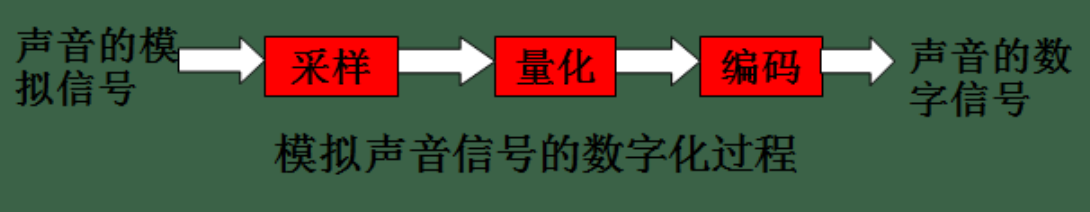
\includegraphics[scale=0.25]{voice_digtial}\\ 
\end{frame}

%%%%%%%%%%%%%%%%%%%%%%%%%%%%%%%%%%%%%%%%
% A frame
%%%%%%%%%%%%%%%%%%%%%%%%%%%%%%%%%%%%%%%%
\begin{frame}[t]{6. 计算机多媒体技术基础} \vspace{20pt}
    ⑴ 采样\\
采样是每隔一定的时间间隔在模拟波形上取一个幅度值,从而得到一系列的声音采样
值,这样就把时间上的连续信号变成时间上的离散信号。\\
⑵ 量化\\
量化是将每个采样点的幅度值以数字存储,量化的位数(即采样精度)表示存放采样
点幅度值的二进制位数。通常量化的位数有 8 位、16 位等。\\
⑶ 编码\\
将采样和量化后的数字数据以一定的格式记录下来。
模拟波形声音被数字化后音频文件的存储量(假定未经压缩)为:
存储量=采样频率×量化位数/8×声道数×时间
其中存储量单位为字节(BYTE)\\

\end{frame}


%%%%%%%%%%%%%%%%%%%%%%%%%%%%%%%%%%%%%%%%
% A frame
%%%%%%%%%%%%%%%%%%%%%%%%%%%%%%%%%%%%%%%%
\begin{frame}[t]{6. 计算机多媒体技术基础} \vspace{20pt}
【单选】用 22.05KHz 的采样频率进行采样,量化位数选用 16 位,则录制 1 分钟的立
体声,需要数据量为( )\\
A.22050 × 16 × 2 × 60 byte\\
B.22050 × 16 × 2 × 60÷8 byte\\
C.22050 × 16 × 60÷8 byte\\
D.22050 × 16 × 60÷8 bit\\
\end{frame}





%%%%%%%%%%%%%%%%%%%%%%%%%%%%%%%%%%%%%%%%
% A frame
%%%%%%%%%%%%%%%%%%%%%%%%%%%%%%%%%%%%%%%%
\begin{frame}[t]{6. 计算机多媒体技术基础} \vspace{20pt}
【单选】用 22.05KHz 的采样频率进行采样,量化位数选用 16 位,则录制 1 分钟的立
体声,需要数据量为( )\\
A.22050 × 16 × 2 × 60 byte\\
B.22050 × 16 × 2 × 60÷8 byte\\
C.22050 × 16 × 60÷8 byte\\
D.22050 × 16 × 60÷8 bit\\
存储量=采样频率×量化位数/8×声道数×时间\\
    () = 22050 * 16/8 * 60 byte\\
答案:B\\
\end{frame}




%%%%%%%%%%%%%%%%%%%%%%%%%%%%%%%%%%%%%%%%
% A frame
%%%%%%%%%%%%%%%%%%%%%%%%%%%%%%%%%%%%%%%%
\begin{frame}[t]{6. 计算机多媒体技术基础} \vspace{20pt}
    6.3 \textbf{图像}\\
    图像(Image)数字化过程:\\

    (1) 采样\\
采样的实质就是用若干个像素(Pixel)点来描述图像,称为图像的分辨率,用点的
“列数×行数”表示。\\

(2) 量化\\
量化是在图像经采样离散化之后,用二进制数来表示这些离散点对应的颜色信息
的过程。\\
(3) 图像编码压缩\\
无损压缩:对图像中的重复信息压缩,无失真。
有损压缩:通过去掉图像细节来压缩图像,有失真。常见的图像文件格式 :\\
位图文件格式(.bmp)
JPEG 文件格式(.jpg 或.jpeg)
GIF 文件格式(.gif)
TIFF 文件格式(.tif 或.tiff)
PSD 文件格式(.psd)\\


\end{frame}


%%%%%%%%%%%%%%%%%%%%%%%%%%%%%%%%%%%%%%%%
% A frame
%%%%%%%%%%%%%%%%%%%%%%%%%%%%%%%%%%%%%%%%
\begin{frame}[t]{6. 计算机多媒体技术基础} \vspace{20pt}
    6.3 \textbf{图像}\\
    \textbf{图像数据量的计算}\\
    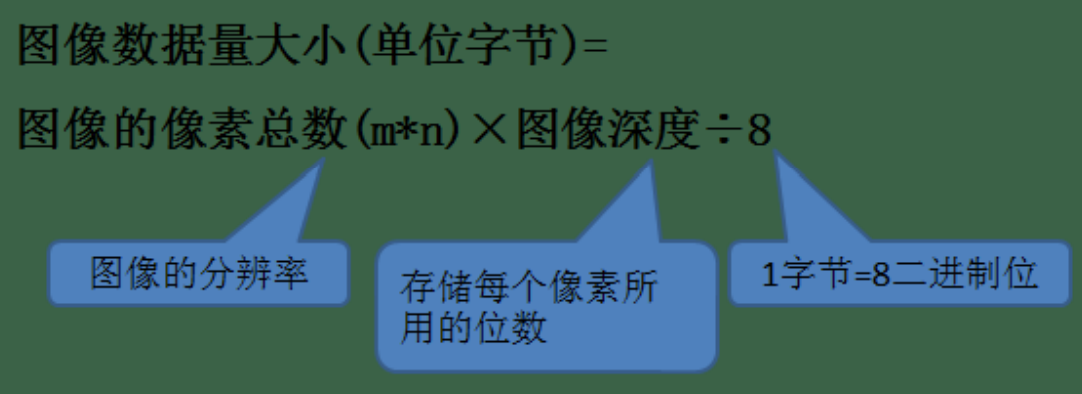
\includegraphics[scale=0.25]{image_data_cal}\\ 
    图像深度确定彩色图像的每个像素可能有的颜色数,决定了彩色图像中可出现的最多
颜色数,若每个像素有 8 位,则最大灰度数目为 2 的 8 次方,即图像能表示 \textbf{256} 种颜
色。\\
\end{frame}

%%%%%%%%%%%%%%%%%%%%%%%%%%%%%%%%%%%%%%%%
% A frame
%%%%%%%%%%%%%%%%%%%%%%%%%%%%%%%%%%%%%%%%
\begin{frame}[t]{6. 计算机多媒体技术基础} \vspace{20pt}
    6.3 \textbf{图像}\\
    【单选】一幅图像的尺寸为 1024×768 像素,颜色深度为 16,则它的未压缩的数据量
为( )。\\
A.1.5MB\\ B.2.0MB\\
C.2.5MB\\ D.3.0MB\\
\end{frame}


%%%%%%%%%%%%%%%%%%%%%%%%%%%%%%%%%%%%%%%%
% A frame
%%%%%%%%%%%%%%%%%%%%%%%%%%%%%%%%%%%%%%%%
\begin{frame}[t]{6. 计算机多媒体技术基础} \vspace{20pt}
    6.3 \textbf{图像}\\
    【单选】一幅图像的尺寸为 1024×768 像素,颜色深度为 16,则它的未压缩的数据量
为( )。\\
A.1.5MB\\ B.2.0MB\\
C.2.5MB\\ D.3.0MB\\
答案:A\\
解析:1024×768 ×16 ÷8 ÷1024 ÷1024=1.5\\
\end{frame}

%%%%%%%%%%%%%%%%%%%%%%%%%%%%%%%%%%%%%%%%
% A frame
%%%%%%%%%%%%%%%%%%%%%%%%%%%%%%%%%%%%%%%%
\begin{frame}[t]{6. 计算机多媒体技术基础} \vspace{20pt}
    6.3 \textbf{图像}\\
    【单选】一幅没有经过数据压缩的能表示 256 种不同颜色的彩色图像,其数据量是
1.25MB,假设它的垂直分辨率是 1024,那么它的水平分辨率为( )\\
A.1024\\ B.1280\\ C.768\\ D.512\\
\end{frame}

%%%%%%%%%%%%%%%%%%%%%%%%%%%%%%%%%%%%%%%%
% A frame
%%%%%%%%%%%%%%%%%%%%%%%%%%%%%%%%%%%%%%%%
\begin{frame}[t]{6. 计算机多媒体技术基础} \vspace{20pt}
    6.3 \textbf{图像}\\
    【单选】一幅没有经过数据压缩的能表示 256 种不同颜色的彩色图像,其数据量是
1.25MB,假设它的垂直分辨率是 1024,那么它的水平分辨率为( )\\
A.1024\\ B.1280\\ C.768\\ D.512\\
答案:B\\
解析:表示 256 种不同颜色,则图像深度为 8,\\
1.25 ×1024 ×1024 × 8/(1024 × 8)=1280\\
\end{frame}



%%%%%%%%%%%%%%%%%%%%%%%%%%%%%%%%%%%%%%%%
% A frame
%%%%%%%%%%%%%%%%%%%%%%%%%%%%%%%%%%%%%%%%
\begin{frame}[t]{6. 计算机多媒体技术基础} \vspace{20pt}
    6.3 \textbf{视频}\\
    视频即运动图像,是由一系列的静态图像按一定的顺序排列组成,每一幅称为帧(Frame)。\\
MPEG 标准:由国际标准化组织(ISO)和国际电工委员会(IEC)联合成立的专家组。是目前
热门的国际标准,用于活动图像的编码。\\
常见的视频文件格式:\\
AVI 格式(.avi)、\\
MPEG 格式(.dat、.vob、.asf 等)、\\
MOV 格式(.mov)、\\
RM 格式 (.rm、.rmvb)、\\
WMV 格式(.wmv)\\
\end{frame}





%%%%%%%%%%%%%%%%%%%%%%%%%%%%%%%%%%%%%%%%
% A frame
%%%%%%%%%%%%%%%%%%%%%%%%%%%%%%%%%%%%%%%%
\begin{frame}[t]{6. 计算机多媒体技术基础} \vspace{20pt}
    6.4 \textbf{多媒体计算机系统的组成}\\
    五、多媒体计算机系统的组成

    \begin{enumerate}
        \item {声卡}:又称音频卡, 是处理音频信号的硬件。\\
        \item {\textbf{视频卡}}:用来支持视频信号(主要指活动彩色图像信号)的输入和输出 。\\
            可实现对语音、图像的采集、压缩和重放。\\
        \item {扫描仪}:常用的图形、图像、文本等信息的输入设备。\\
        \item {声卡}:又称音频卡, 是处理音频信号的硬件。\\
        \item {数码相机与数码摄像机 }:获取电子图像、动态影像 。\\
    \end{enumerate}
\end{frame}



%%%%%%%%%%%%%%%%%%%%%%%%%%%%%%%%%%%%%%%%
% A frame
%%%%%%%%%%%%%%%%%%%%%%%%%%%%%%%%%%%%%%%%
\begin{frame}[t]{6. 计算机多媒体技术基础} \vspace{20pt}

    练习题\\
    【单选】在多媒体技术中,运动图像压缩编码的国际标准是( )\\
    A. JPEG\\
    B. AVI\\
    C. MPEG\\
    D. MP3\\
\end{frame}


%%%%%%%%%%%%%%%%%%%%%%%%%%%%%%%%%%%%%%%%
% A frame
%%%%%%%%%%%%%%%%%%%%%%%%%%%%%%%%%%%%%%%%
\begin{frame}[t]{6. 计算机多媒体技术基础} \vspace{20pt}

    练习题\\
    【单选】在多媒体技术中,运动图像压缩编码的国际标准是( )\\
    A. JPEG\\
    B. AVI\\
    C. MPEG\\
    D. MP3\\
    答案:C\\
\end{frame}

%%%%%%%%%%%%%%%%%%%%%%%%%%%%%%%%%%%%%%%%
% A frame
%%%%%%%%%%%%%%%%%%%%%%%%%%%%%%%%%%%%%%%%
\begin{frame}[t]{6. 计算机多媒体技术基础} \vspace{20pt}

    练习题\\
    【单选】Windows XP 操作系统自身携带的媒体播放器是( )\\
    A. Qvod\\
    B. Windows Media Player\\
    C. Rinamp\\
    D. Realplayer\\
    答案:B\\




\end{frame}














\end{document}
